\startchapter{Hardware Trojans}
\label{chapter:hardwareTrojans}

\newlength{\savedunitlength}
\setlength{\unitlength}{2em}
\section{Background}

\section{Topology}
The discussion, detection and evaluation of hardware trojans requires a comprehensive means of describing them.
Several hardware trojan taxonomies have been proposed~\cite{taxonomy1, taxonomy2, taxonomy3, taxonomy4}.
In~\cite{taxonomy1}, trojans were organized based solely on their activation mechanisms.
A taxonomy based on the location, activation and action of a trojan was presented in \cite{taxonomy2}, \cite{taxonomy3}.
However, these approaches do not consider the manufacturing process.
Another taxonomy was proposed in~\cite{taxonomy4} which employs five categories: insertion, abstraction, activation, effect, and location.
While this is more extensive than previous approaches, it fails to account for the physical characteristics of a trojan.
An additional taxonomy was proposed in~\cite{samerAttribute} which considers all attributes a hardware trojan may posses.
This taxonomy is the most comprehensive and was selected as the means of description for this work.
\begin{figure}
	\centering
	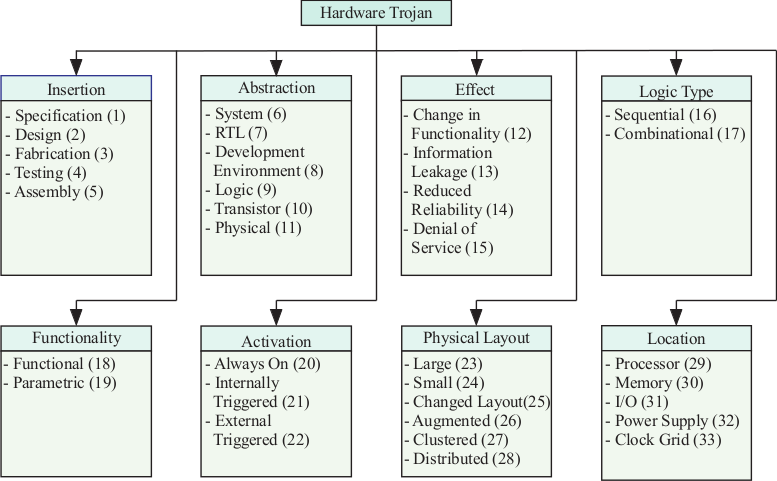
\includegraphics[width=1.0\linewidth]{figures/HW_trojan}
	\caption{The thirty-three attributes of the hardware trojan taxonomy in~\cite{samerAttribute}.}
	\label{fig:HW_trojan}
\end{figure}
It is comprised of thirty-three attributes organized into eight categories as shown in Fig.~\ref{fig:HW_trojan}.
These categories can be arranged into the following four levels as indicated in Fig.~\ref{fig:trojan_life_cycle}.
\begin{enumerate}
	\item The \textbf{insertion} (chip life-cycle) level/category comprises the attributes pertaining to the IC production stages.
	\item The \textbf{abstraction} level/category corresponds to where in the IC abstraction the trojan is introduced.
	\item The \textbf{properties} level comprises the behavior and physical characteristics of the trojan.
	\item The \textbf{location} level/category corresponds to the location of the trojan in the IC.
\end{enumerate}
The properties level consists of the following categories.
\begin{itemize}
	\item The \textbf{effect} describes the disruption or effect a trojan has on the system.
	\item The \textbf{logic type} is the circuit logic that triggers the trojan, either combinational or sequential.
	\item The \textbf{functionality} differentiates between trojans which are functional or parametric.
	\item The \textbf{activation} differentiates between trojans which are always on or triggered.
	\item The \textbf{layout} is based on the physical characteristics of the trojan.
\end{itemize}
\begin{figure}
	\centering
	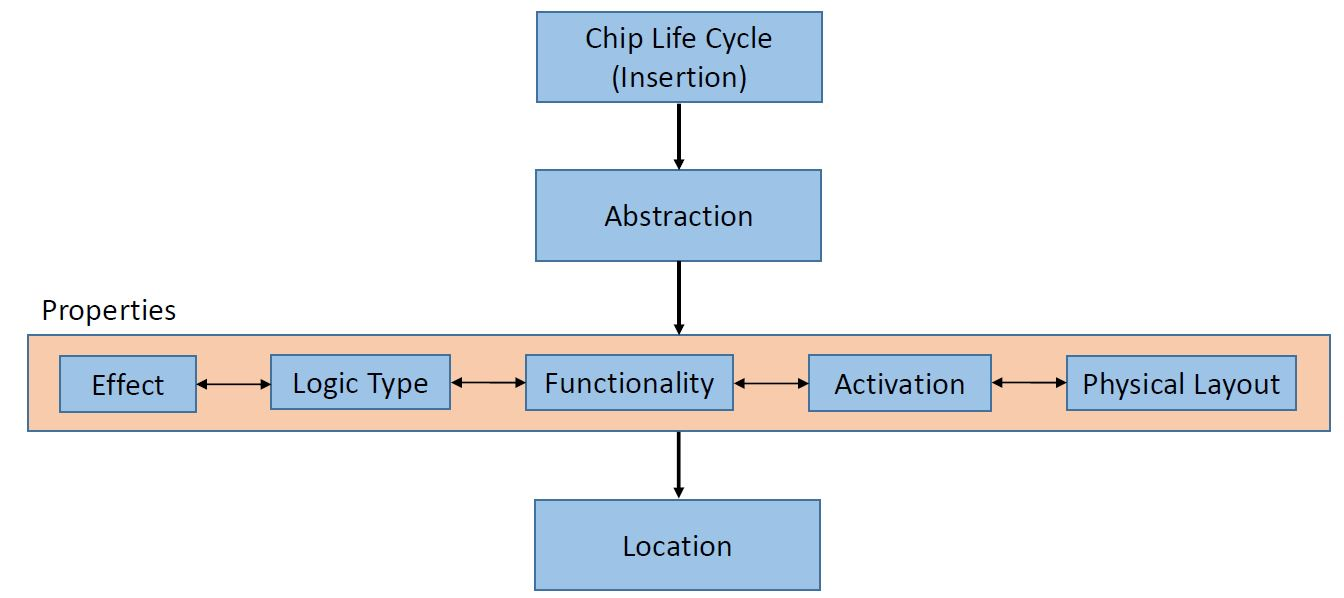
\includegraphics[width=0.8\linewidth]{figures/trojan_life_cycle}
	\caption{The hardware trojan levels \cite{samerAttribute}.}
	\label{fig:trojan_life_cycle}
\end{figure}
\setlength{\unitlength}{\savedunitlength}